\documentclass{article}

\usepackage{booktabs}
\usepackage{multirow}
\usepackage{amsmath}
\usepackage{hyperref}
\usepackage{overpic}
\usepackage{amssymb}
\usepackage{cuted}
\usepackage{array}
\usepackage{booktabs}
\usepackage{caption}
\usepackage[inline]{enumitem}
\usepackage{xcolor}
\usepackage[accepted]{dlaiml2026}

%%% STUDENTS: FILL IN WITH YOUR OWN INFORMATION
\dlaititlerunning{Latent Dynamics and Efficient Inference in Tiny Recursive Models}

\begin{document}

\twocolumn[
%%% STUDENTS: FILL IN WITH YOUR OWN INFORMATION
\dlaititle{Latent Dynamics and Efficient Inference in Tiny Recursive Models}

\begin{center}\today\end{center}

\begin{dlaiauthorlist}
%%% STUDENTS: FILL IN WITH YOUR OWN INFORMATION
\dlaiauthor{Davide Perniconi}{}
\end{dlaiauthorlist}

%%% STUDENTS: FILL IN WITH YOUR OWN INFORMATION
\dlaicorrespondingauthor{Davide Perniconi}{perniconi.1889270@studenti.uniroma1.it}

\vskip 0.3in
]

\printAffiliationsAndNotice{}

\begin{abstract}

Tiny Recursive Model (TRM) is a recent recursive architecture that outperforms frontier LLMs on reasoning tasks.
Despite being called ``tiny'', TRMs require many sequential steps to produce accurate predictions on non-trivial problems.
Furthermore, a recent extension trades off even more inference time for accuracy by requiring dozens of parallel rollouts.
At the same time, the internal evolution of TRM hidden states remains largely unexplored.
This work is twofold: first, it characterizes the geometry of the latent reasoning space of TRMs; second, it addresses the inference-time bottleneck by applying an acceleration-based early stopping criterion and evaluating its impact.

\end{abstract}


% ------------------------------------------------------------------------------
\section{Related Work}
The work is grounded in recent advancements in latent reasoning architectures: \begin{enumerate*}[label=(\roman*)]
\item \textbf{Tiny Recursive Model (TRM):}
\citet{trm} simplifies the biology-inspired HRM architecture \cite{hrm} by iteratively processing hidden states through a single 2-layer Transformer with deep supervision,
\item \textbf{Geometric metrics and early stopping:}
\citet{latent-dynamics} show that internal representations within recurrent Transformer blocks evolve through a combination of fine-grained local refinements and larger-scale drift, and introduces geometric metrics to compare different early-exit mechanisms,
\item \textbf{Probabilistic TRM (PTRM):}
\citet{ptrm} propose a simple training-free extension that blindly injects noise during recursion. Although PTRM achieves substantial accuracy gains, it significantly increases inference costs by requiring up to 100 parallel rollouts per sample.
\end{enumerate*}
The \textbf{main contributions} of this work are: \begin{enumerate*}[label=(\roman*)]
\item implementation from scratch of the TRM (both MLP-Mixer and Attention variants),
\item study of both reasoning and solution latents ($y$ and $z$),
\item implementation of acceleration-based early stopping to reduce inference time, and
\item experimental investigation of Matryoshka Representation Learning imposed on $y$.
\end{enumerate*}


% ------------------------------------------------------------------------------
\section{Method}
TRMs were trained both with and without \textbf{Matryoshka Representation Learning} \cite{mrl}.
For the geometric analysis, the latent trajectories were studied via \textbf{PCA} for visualization, and the metrics introduced in \cite{latent-dynamics} were computed.
The trained models were evaluated and the resulting latent trajectories were recorded for direct inspection of the internal computation process. Additional trajectories were collected from the publicly available ARC-AGI checkpoints \footnote{ARC-AGI checkpoins available \href{https://huggingface.co/arcprize/trm_arc_prize_verification}{here}.}.
Finally, TRM was extended with the early stopping criterion based on the unnormalized acceleration (see Equation~\ref{eq:acceleration}) with two-hit check \cite{latent-dynamics}.
The objective is to achieve approximately the same accuracy obtained using all supervision steps ($N_{\text{sup}} = 16$) while reducing the average number of iterations during inference.
% ------------------------------------------------------------------------------

\section{Experimental Results}

\paragraph{Setup}
We train TRMs on Maze 5x5, Maze 10x10 (generated using the \texttt{maze-dataset} library \cite{maze-dataset}), and Sudoku 9x9 (10k samples with difficulty $\leq 2$ sourced from Hugging Face\footnote{Sudoku $9\times9$ samples were filtered from \href{https://huggingface.co/datasets/Ritvik19/Sudoku-Dataset}{this dataset}.}).
For all tasks, the internal recursive block of the TRM is configured as a compact 2-layer Transformer with
$N_{\text{sup}} = 16$ supervision steps, $T = 4$ deep recursion steps, and $n = 8$ latent recursion steps. All high-dimensional latent trajectories are analyzed via Principal Component Analysis (PCA).

\paragraph{Effect of MRL}
As shown in Table~\ref{tab:eval-results}, MRL yields virtually identical performance to the full latent representation, except for the Sudoku 9x9 MLP-Mixing configuration.
MRL can therefore serve as a diagnostic probe for estimating the intrinsic dimensionality of the reasoning manifold without interfering with the deep supervision mechanism.
Even when considering only the first few dimensions of $y$, the solution can be approximated effectively. For Maze $5\times5$, \textit{using only the first dimension}, Token Accuracy remains around 83\% (Table~\ref{tab:token-accuracy}).
Empirical trials with acceleration-based early stopping revealed identical stopping patterns for MRL-enhanced and standard TRMs.
Given this equivalence, the early stopping experiments reported in Table~\ref{tab:ea-results} focus exclusively on non-MRL models.

\paragraph{Difference Between Reasoning and Solutions}
Within each deep supervision step, the features of $z$ exhibit high-frequency oscillations across the internal $n$ computational cycles before eventually aligning with the solution state $y$.
This behavior makes $y$ more suitable than $z$ for defining a stable stopping criterion.
This dynamic is illustrated in Figures~\ref{fig:sudoku9x9-metrics} and~\ref{fig:maze5x5-metrics}.

\paragraph{Two-Regime Updates}
Examination of individual trajectories (Figures~\ref{fig:maze5x5-traj} and~\ref{fig:sudoku9x9-traj}) reveals two distinct computational phases.
Once a macroscopic \textbf{coarse solution} emerges during the initial recursive steps, the network transitions into a localized \textbf{fine refinement} regime.
This topological behavior provides empirical support for the two-scale latent dynamics framework proposed in \cite{latent-dynamics}, suggesting that TRMs refine solutions incrementally rather than repeatedly altering their semantic interpretation at each step.

\paragraph{Trajectory Clustering}
Simultaneous analysis of multiple trajectories from initialization to convergence (see the ARC-AGI results in Figures~\ref{fig:agi-v1-clusters} and~\ref{fig:agi-v2-clusters}) reveals a clear topological organization.
Latent representations do not diffuse chaotically; instead, they progressively \textbf{accumulate and converge toward well-defined attractor regions} within the manifold, indicating that the reasoning process evolves toward stable fixed points.
This observation may be related to ideas underlying Deep Equilibrium Models (DEQ) \cite{deq} and the Implicit Function Theorem (IFT) discussed by \citet{hrm}.

\paragraph{Early Stopping}
Given this geometry, a halting mechanism becomes theoretically justified.
Table~\ref{tab:ea-results} shows that acceleration-based early stopping substantially reduces the average number of computational steps across all tasks without sacrificing accuracy (see Table~\ref{tab:eval-results} for comparison).
Crucially, the unnormalized acceleration provides a \textbf{more robust stopping signal} than the normalized variant (Equations~\ref{eq:acceleration} and~\ref{eq:norm-acceleration}).
During the initial phase, updates $\Delta^{(k)}$ are large, whereas near convergence $\Vert \Delta^{(k)} \Vert_2 \rightarrow 0$ (localized refinements).
In this transition between the two latent regimes, the unnormalized acceleration cleanly drops to zero because successive updates become identical.
Conversely, for the normalized metric, both the numerator and the denominator vanish simultaneously. As a result, the normalized acceleration curve plateaus with severe oscillations and fails to reliably signal convergence, as visually demonstrated in Figures~\ref{fig:maze5x5-traj} and~\ref{fig:sudoku9x9-traj}.

\begin{strip}
\begin{center}
\footnotesize
\setlength{\tabcolsep}{5pt}
    \captionof{table}{
        Exact accuracy (\%) results. "Halted" (\%) reports the percentage of samples that skipped at least
        one step. "Avg steps" means the average step performed (16 implies no early exiting). 
        "(attn)" means that the TRM used Attention instead of MLP-Mixing.
    }
    \label{tab:ea-results}
    \begin{tabular}{l ccc ccc ccc}
    \toprule
    & \multicolumn{3}{c}{$\tau = 0.5$}
    & \multicolumn{3}{c}{$\tau = 0.8$}
    & \multicolumn{3}{c}{$\tau = 1.0$} \\
    \cmidrule(lr){2-4} \cmidrule(lr){5-7} \cmidrule(lr){8-10}
    Dataset
    & Accuracy & Halted & Avg steps
    & Accuracy & Halted & Avg steps
    & Accuracy & Halted & Avg steps \\
    \midrule
    Maze 5x5          & 96 & 44 & 12 & 95 & 84 & 6.4 & 96 & 100 & 2 \\
    Maze 10x10        & 96 & 38 & 12 & 97 & 71 & 7.8 & 97 & 100 & 2 \\
    Sudoku 9x9        & 82 & 71 & 9 & 80 & 90 & 5.3 & 77 & 100 & 2 \\
    Sudoku 9x9 (attn) & 94 & 49 & 11 & 94 & 84.2 & 7 & 93 & 100 & 2 \\
    \bottomrule
    \end{tabular}
\end{center}
\end{strip}


\section{Conclusion and Future Work}

We investigated the latent dynamics of TRMs, identifying a two-scale geometric regime in which, once a coarse macroscopic solution is established, the trajectory enters a localized refinement phase.
We further showed that the more stable unnormalized acceleration-based early stopping criterion reduces inference-time computation without sacrificing performance.
Additionally, we demonstrated that MRL provides an effective tool for monitoring the intrinsic dimensionality of the reasoning space.
Several directions remain open for future research:
\begin{enumerate*}[label=(\roman*)]
\item can the latent reasoning space learned on Sudoku be transferred to related tasks such as KenKen or Latin squares?
\item can trajectories be accelerated through autoregressive generation or direct future-state prediction?
\item in tasks admitting multiple solutions, can TRMs become truly probabilistic by returning multiple valid answers?
\end{enumerate*}
% \begin{enumerate*}[label=(\roman*)]
% \item \textbf{Domain Transfer and MRL Probing:} future work will investigate whether the latent reasoning space acquired on Sudoku can be transferred to similar tasks such as KenKen or Latin Squares, using MRL to quantify the geometric overlap of the manifolds.
% \item \textbf{Trajectory prediction:} autoregressive trajectory generation or future latents prediction at time $k$ given previous $y^{0:k-1}$ and $z^{0:k-1}$
% \item \textbf{Generative Diversity in Multi-Solution Tasks:} many reasoning benchmarks allow for multiple valid outputs. Replacing the "brute-force" parallel rollouts of PTRMs \cite{ptrm} with a calibrated temperature parameter could transform the architecture into a probabilistic model capable of exploring distinct solution paths.
% \end{enumerate*}


\section{Statement on the use of AI}

AI tools were used to summarize and analyze relevant scientific literature, assist with model implementation, and generate plotting scripts.
LLMs were also used to organize the obtained results and improve the clarity, conciseness, and academic style of the report.

\bibliography{references.bib}
\bibliographystyle{dlaiml2026}

\section*{Limitations}
The primary limitation of this study introduces a stark computational trade-off between the inherent overhead of the TRM architecture and the hardware resources required to validate early stopping.
Paradoxically, evaluating an early stopping criterion demands complex, high-dimensional reasoning problems that natively require a large number of supervision steps ($N_{\text{sup}}$) to justify the computational exit.
However, the sequential nature of this recursive mechanism creates a severe computation bottleneck. Consequently, testing the maximum recurrence bounds proved computationally intractable within standard cloud environments like Google Colab or Kaggle.
Furthermore, our geometric exploration was bounded by the public checkpoints released by the original authors. Because they exclusively provided pre-trained artifacts for the ARC-AGI benchmarks, other tasks like Sudoku 9x9 Extreme and Maze 30x30 Hard remained inaccessible for trajectory analysis.
Finally, due to strict memory and storage constraints when logging massive sequences of intermediate hidden states across numerous steps, the collective study of ARC-AGI latent trajectories had to be restricted to a bounded subset of samples, scaled to the absolute maximum threshold permitted by the available hardware constraints, which nevertheless provided a sufficiently dense corpus to isolate and verify stable convergence behaviors.


\clearpage
\onecolumn

\section*{Appendix}


\subsection*{Formulas}

The $\Delta$ factor used for acceleration is computed on solution latents $y$ and defined as ($k$ denotes supervision step):

\begin{equation}
    \label{eq:delta}
    \Delta^{(k)} = y^{(k+1)} - y^{(k)}
\end{equation}

The standard unnormalized acceleration is defined as :

\begin{equation}
    \label{eq:acceleration}
    a^{(k)} = \big\lVert \Delta^{(k)} - \Delta^{(k-1)} \big\rVert_2
\end{equation}

The normalized acceleration (drop-in replacement) is defined as:

\begin{equation}
    \label{eq:norm-acceleration}
    \hat{a}^{(k)} = \frac{\left\|\Delta^{(k)} - \Delta^{(k-1)}\right\|_{2}}
    {\left\|\Delta^{(k)}\right\|_{2} + \left\|\Delta^{(k-1)}\right\|_{2} + \varepsilon}
    \in [0,2]
\end{equation}


\subsection*{Results without early stopping}

Below are reported the results obtained when using different supervision steps ($N_{\mathrm{sup}}$). Maze tasks appear to be
solvable with just one supervision step while Sudoku requires at least $N_{\mathrm{sup}} = 2$.

\begin{center}
\footnotesize
\setlength{\tabcolsep}{5pt}
    \captionof{table}{
        Exact accuracy (\%) achieved across datasets with and without MRL. "(attn)" means that attention instead of MLP-Mixing was used.
        The numbers below "no MRL" represent the full hidden size.
    }
    \label{tab:eval-results}
    \begin{tabular}{c ccccccccccccccccc}
    \toprule
    \multirow{4}{*}{$N_{\mathrm{sup}}$} &
    \multicolumn{4}{c}{Maze 5x5} &
    \multicolumn{5}{c}{Maze 10x10} &
    \multicolumn{4}{c}{Sudoku 9x9} &
    \multicolumn{4}{c}{Sudoku 9x9 (attn)} \\
    \cmidrule(lr){2-5}
    \cmidrule(lr){6-10}
    \cmidrule(lr){11-14}
    \cmidrule(lr){15-18}
    &
    \multicolumn{3}{c}{MRL} & \multicolumn{1}{c}{no MRL} &
    \multicolumn{4}{c}{MRL} & \multicolumn{1}{c}{no MRL} &
    \multicolumn{3}{c}{MRL} & \multicolumn{1}{c}{no MRL} &
    \multicolumn{3}{c}{MRL} & \multicolumn{1}{c}{no MRL} \\
    \cmidrule(lr){2-4} \cmidrule(lr){5-5}
    \cmidrule(lr){6-9} \cmidrule(lr){10-10}
    \cmidrule(lr){11-13} \cmidrule(lr){14-14}
    \cmidrule(lr){15-17} \cmidrule(lr){18-18}
    &
    4 & 8 & 16 & 16 &
    4 & 8 & 16 & 32 & 32 &
    4 & 8 & 16 & 16 &
    16 & 64 & 128 & 128 \\
    \midrule
    1  & 0.98 & 0.98 & 0.98 & 0.87 &
        1 & 1 & 1 & 1 & 0.98 &
        0.56 & 0.59 & 0.59 & 0.61 &
        0.61 & 0.61 & 0.61 & 0.69 \\
    2  & 0.98 & 0.98 & 0.98 & 0.96 &
        1 & 1 & 1 & 1 & 0.97 &
        0.74 & 0.74 & 0.74 & 0.77 &
        0.92 & 0.92 & 0.92 & 0.93 \\
    4  & 0.98 & 0.98 & 0.98 & 0.96 &
        1 & 1 & 1 & 1 & 0.97 &
        0.77 & 0.77 & 0.77 & 0.82 &
        0.94 & 0.94 & 0.94 & 0.94 \\
    8  & 0.98 & 0.98 & 0.98 & 0.95 &
        1 & 1 & 1 & 1 & 0.97 &
        0.77 & 0.77 & 0.77 & 0.82 &
        0.94 & 0.94 & 0.94 & 0.94 \\
    16 & 0.99 & 0.99 & 0.99 & 0.95 &
        1 & 1 & 1 & 1 & 0.97 &
        0.77 & 0.77 & 0.77 & 0.82 &
        0.94 & 0.94 & 0.94 & 0.94 \\
    \bottomrule
    \end{tabular}
\end{center}

\begin{center}
\footnotesize
\setlength{\tabcolsep}{5pt}
\captionof{table}{
    Token accuracy (\%) achieved across datasets with MRL. Results refer to $N_{\mathrm{sup}} = 16$.
    Below each task are reported the MRL dimensions used for prediction.\\
}
\label{tab:token-accuracy}
\begin{tabular}{ccccc ccccc cccc cccc}
\toprule
\multicolumn{5}{c}{Maze 5x5} &
\multicolumn{5}{c}{Maze 10x10} &
\multicolumn{3}{c}{Sudoku 9x9} &
\multicolumn{4}{c}{Sudoku 9x9 (attn)} \\

\cmidrule(lr){1-5}
\cmidrule(lr){6-10}
\cmidrule(lr){11-13}
\cmidrule(lr){14-17}

1 & 2 & 4 & 8 & 16 &
2 & 4 & 8 & 16 & 32 &
4 & 8 & 16 &
16 & 32 & 64 & 128 \\

\midrule

82.8 & 98.75 & 99.9 & 99.9 & 99.9 &
99.7 & 1 & 1 & 1 & 1 &
96.2 & 96.25 & 96.3 &
98.74 & 98.73 & 98.73     & 98.73 \\

\bottomrule
\end{tabular}
\end{center}


\subsection*{Plots}

In the following, plots that describe what happens inside reasoning latents, across supervision steps, are presented.
Figure~\ref{fig:sudoku9x9-metrics}, Figure~\ref{fig:sudoku9x9_mrl-metrics}, Figure~\ref{fig:maze5x5-metrics} and Figure~\ref{fig:maze5x5_mrl-metrics} show:
\begin{itemize}
    \item Average magnitude of $\Delta^{(k)}$ step values.
    \item Average step orthogonality $\cos \angle\!\bigl(\Delta^{(k)},\ \Delta^{(k-1)}\bigr)$.
    \item Average normalized acceleration (see Equation~\ref{eq:norm-acceleration}).
\end{itemize}
Figure~\ref{fig:agi-v1-clusters} and figure~\ref{fig:agi-v2-clusters} presents the trajectories generated by the TRM during the recurrent steps and projects them into 3D (inputs comes from ARC-AGI benchmark series).
Finally, figure~\ref{fig:maze5x5-traj} and Figure~\ref{fig:sudoku9x9-traj} show a random sampled trajectory and its evolution with respect to unnormalized and normalized acceleration values.


\subsubsection*{Sudoku 9x9 Metrics}

\begin{center}
    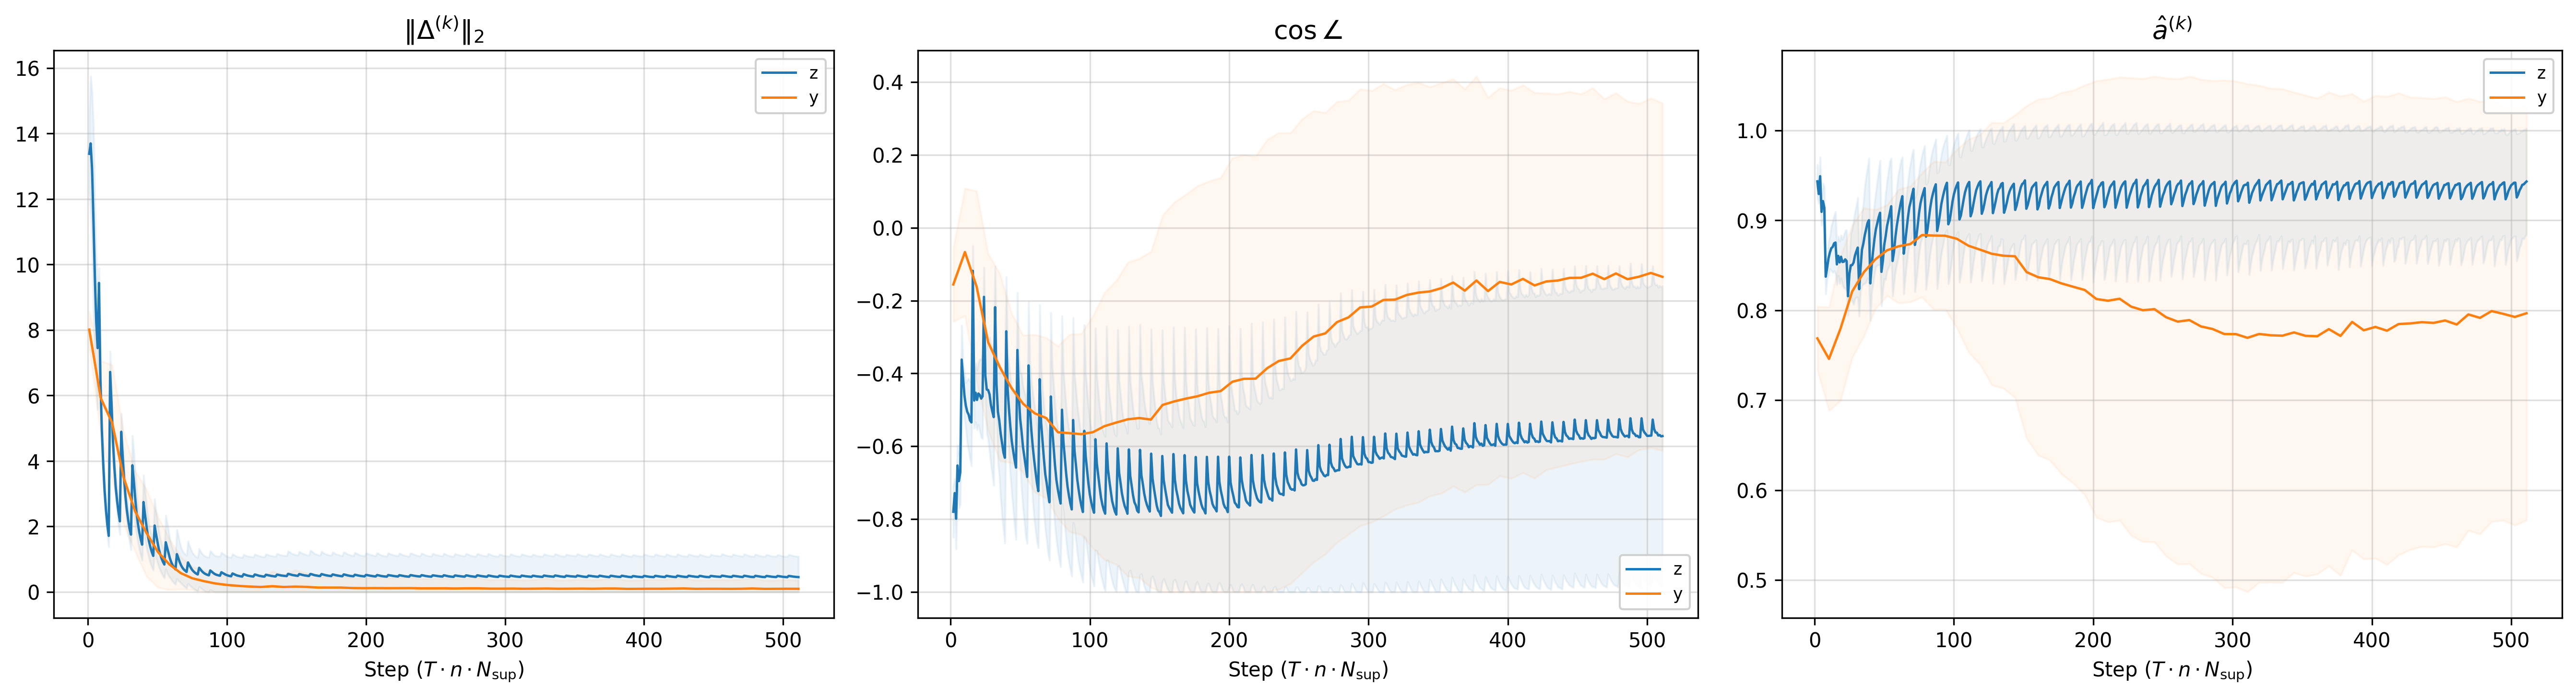
\includegraphics[width=0.98\linewidth]{./figures/sudoku9x9_metrics.png}
    \captionof{figure}{Sudoku 9x9 average geometric metrics}
    \label{fig:sudoku9x9-metrics}

    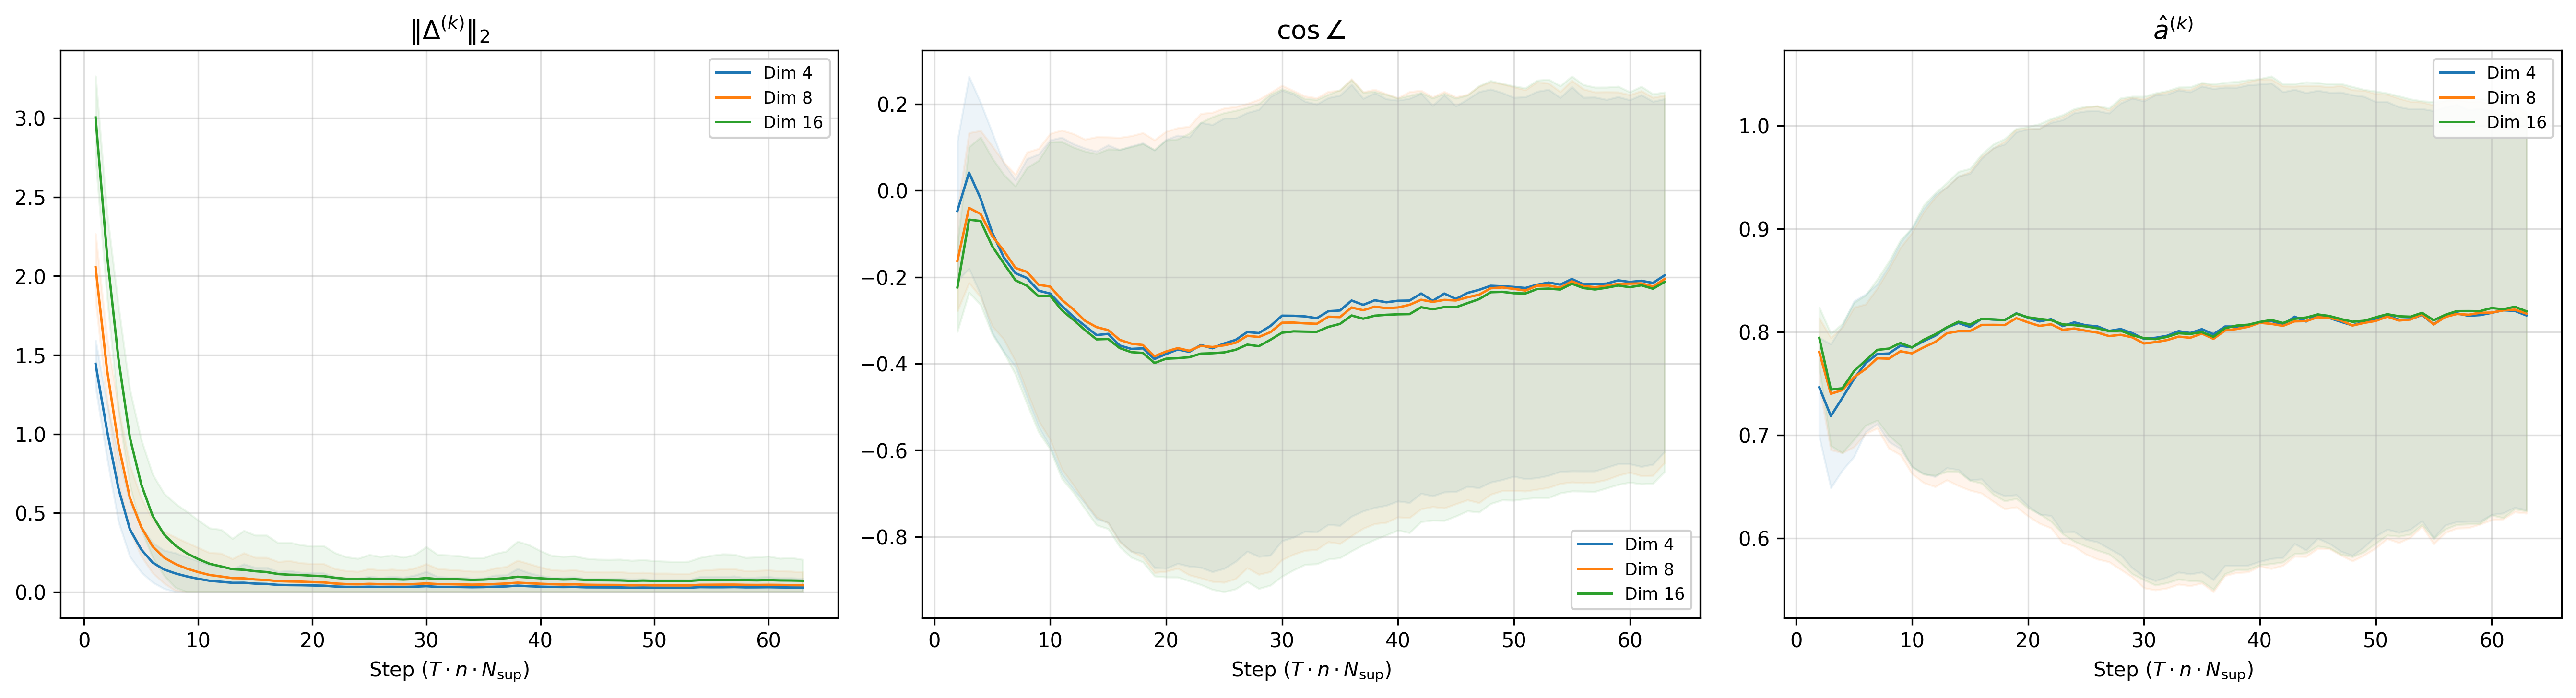
\includegraphics[width=0.98\linewidth]{./figures/sudoku9x9_mrl_metrics.png}
    \captionof{figure}{Sudoku 9x9 MRL average geometric metrics}
    \label{fig:sudoku9x9_mrl-metrics}
\end{center}


\subsubsection*{Maze 5x5 Metrics}

\begin{center}
    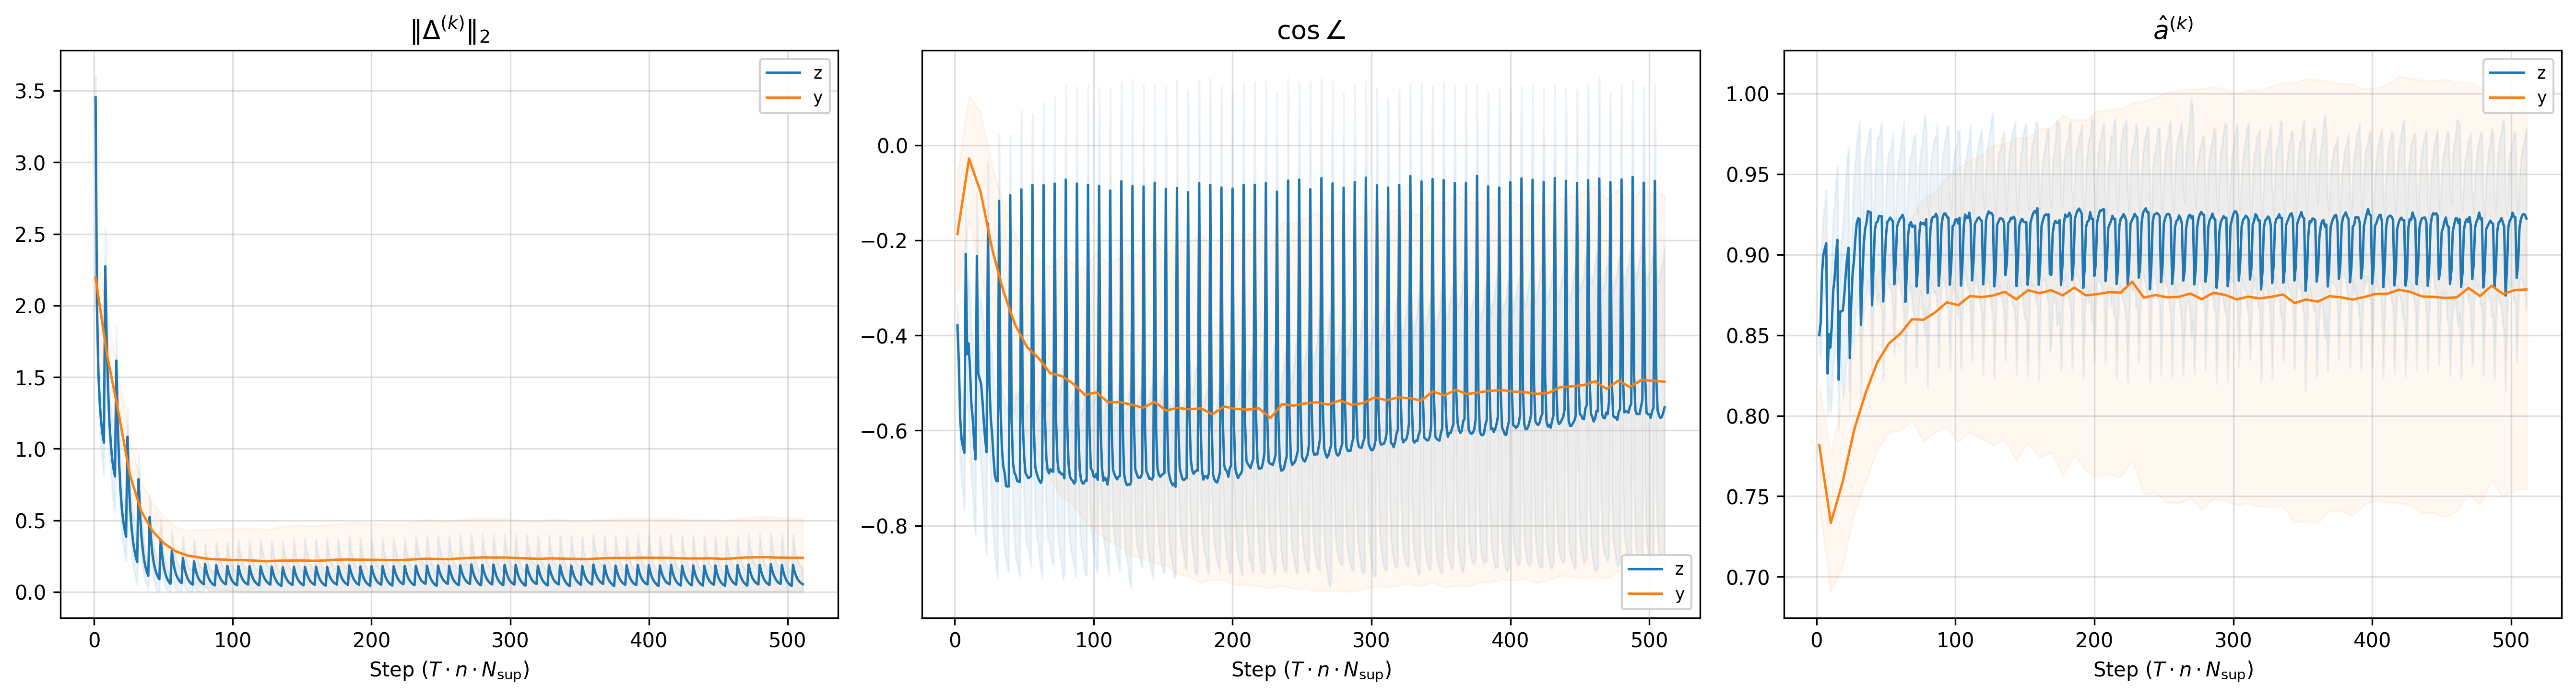
\includegraphics[width=0.98\linewidth]{./figures/maze5x5_metrics.png}
    \captionof{figure}{Maze 5x5 average geometric metrics}
    \label{fig:maze5x5-metrics}


    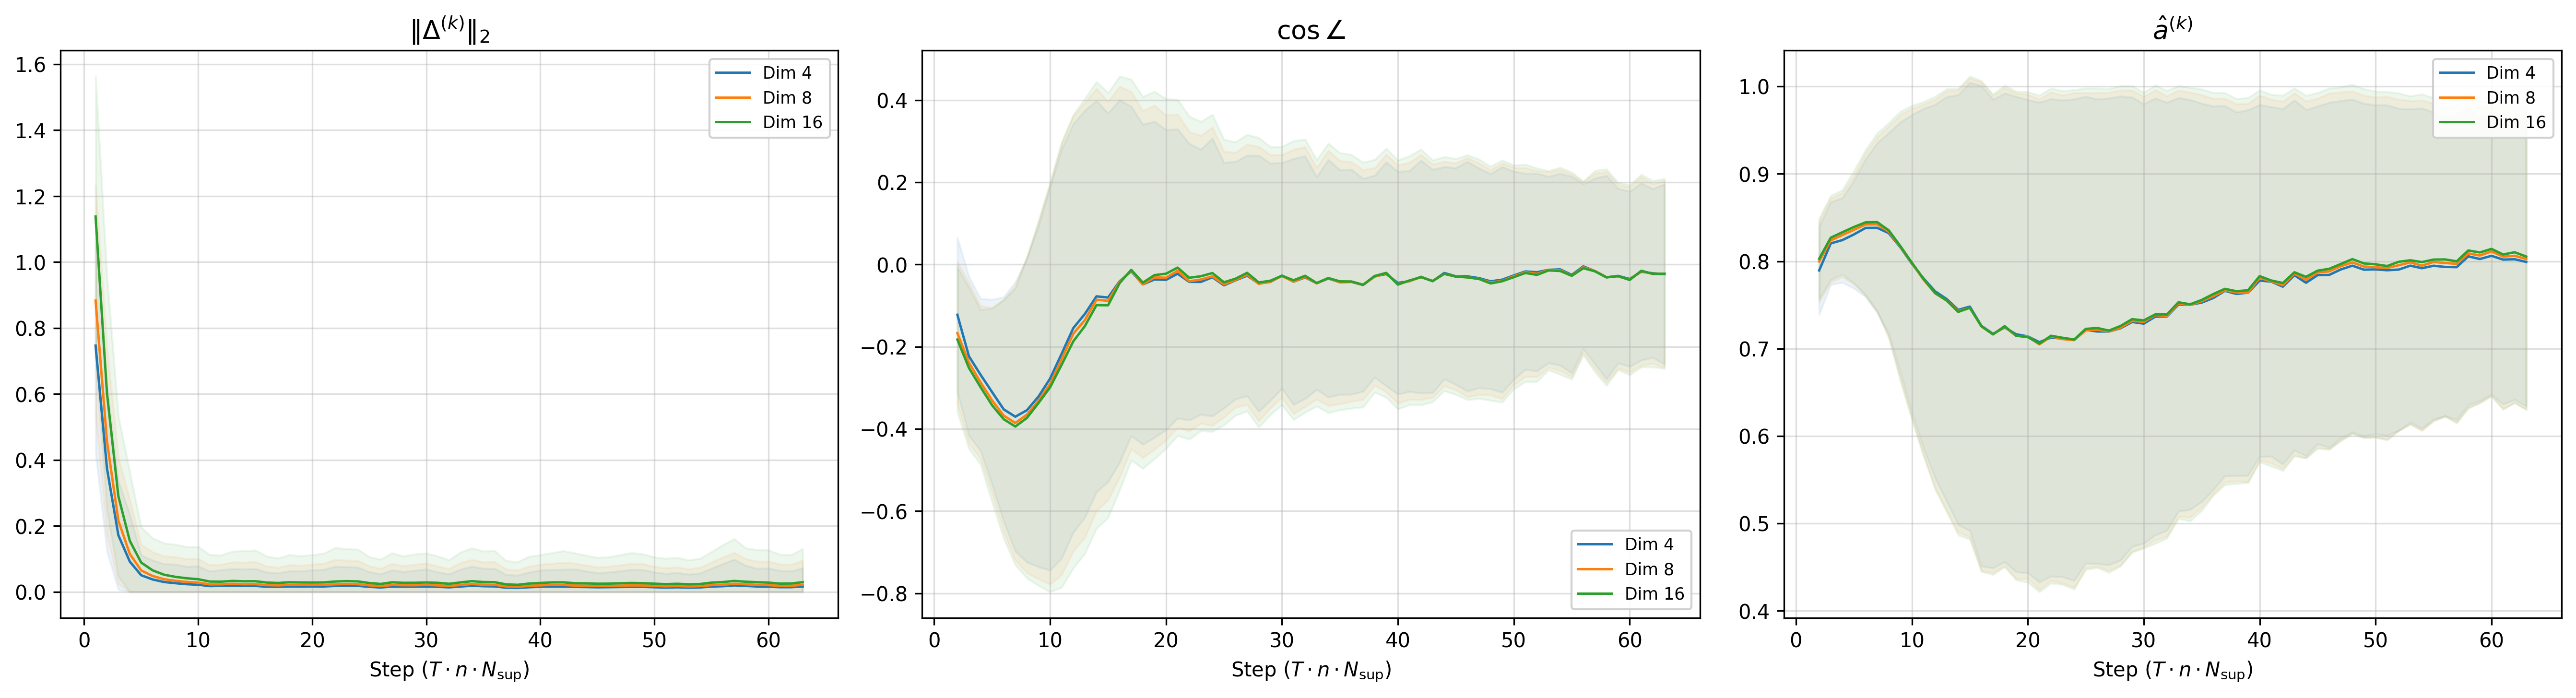
\includegraphics[width=0.98\linewidth]{./figures/maze5x5_mrl_metrics.png}
    \captionof{figure}{Maze 5x5 MRL average geometric metrics}
    \label{fig:maze5x5_mrl-metrics}
\end{center}

\subsubsection*{ARC-AGI Clusters}

The trajectories used for the following plots are collected during evaluation on the validation/test splits, with shape $\texttt{Samples} \times \texttt{Steps} \times \texttt{Seq len} \times \texttt{Hidden size}$. At each supervision step, the representation $y$ is averaged across tokens to obtain a single global representation of the puzzle.
A three-dimensional PCA projection is then fitted jointly on the representations from all trajectories and supervision steps. This yields a shared coordinate system in which trajectories can be visualized and directly compared within the same compressed space.
Colors denote the supervision step, thereby highlighting the temporal progression of the representations.

\begin{center}
    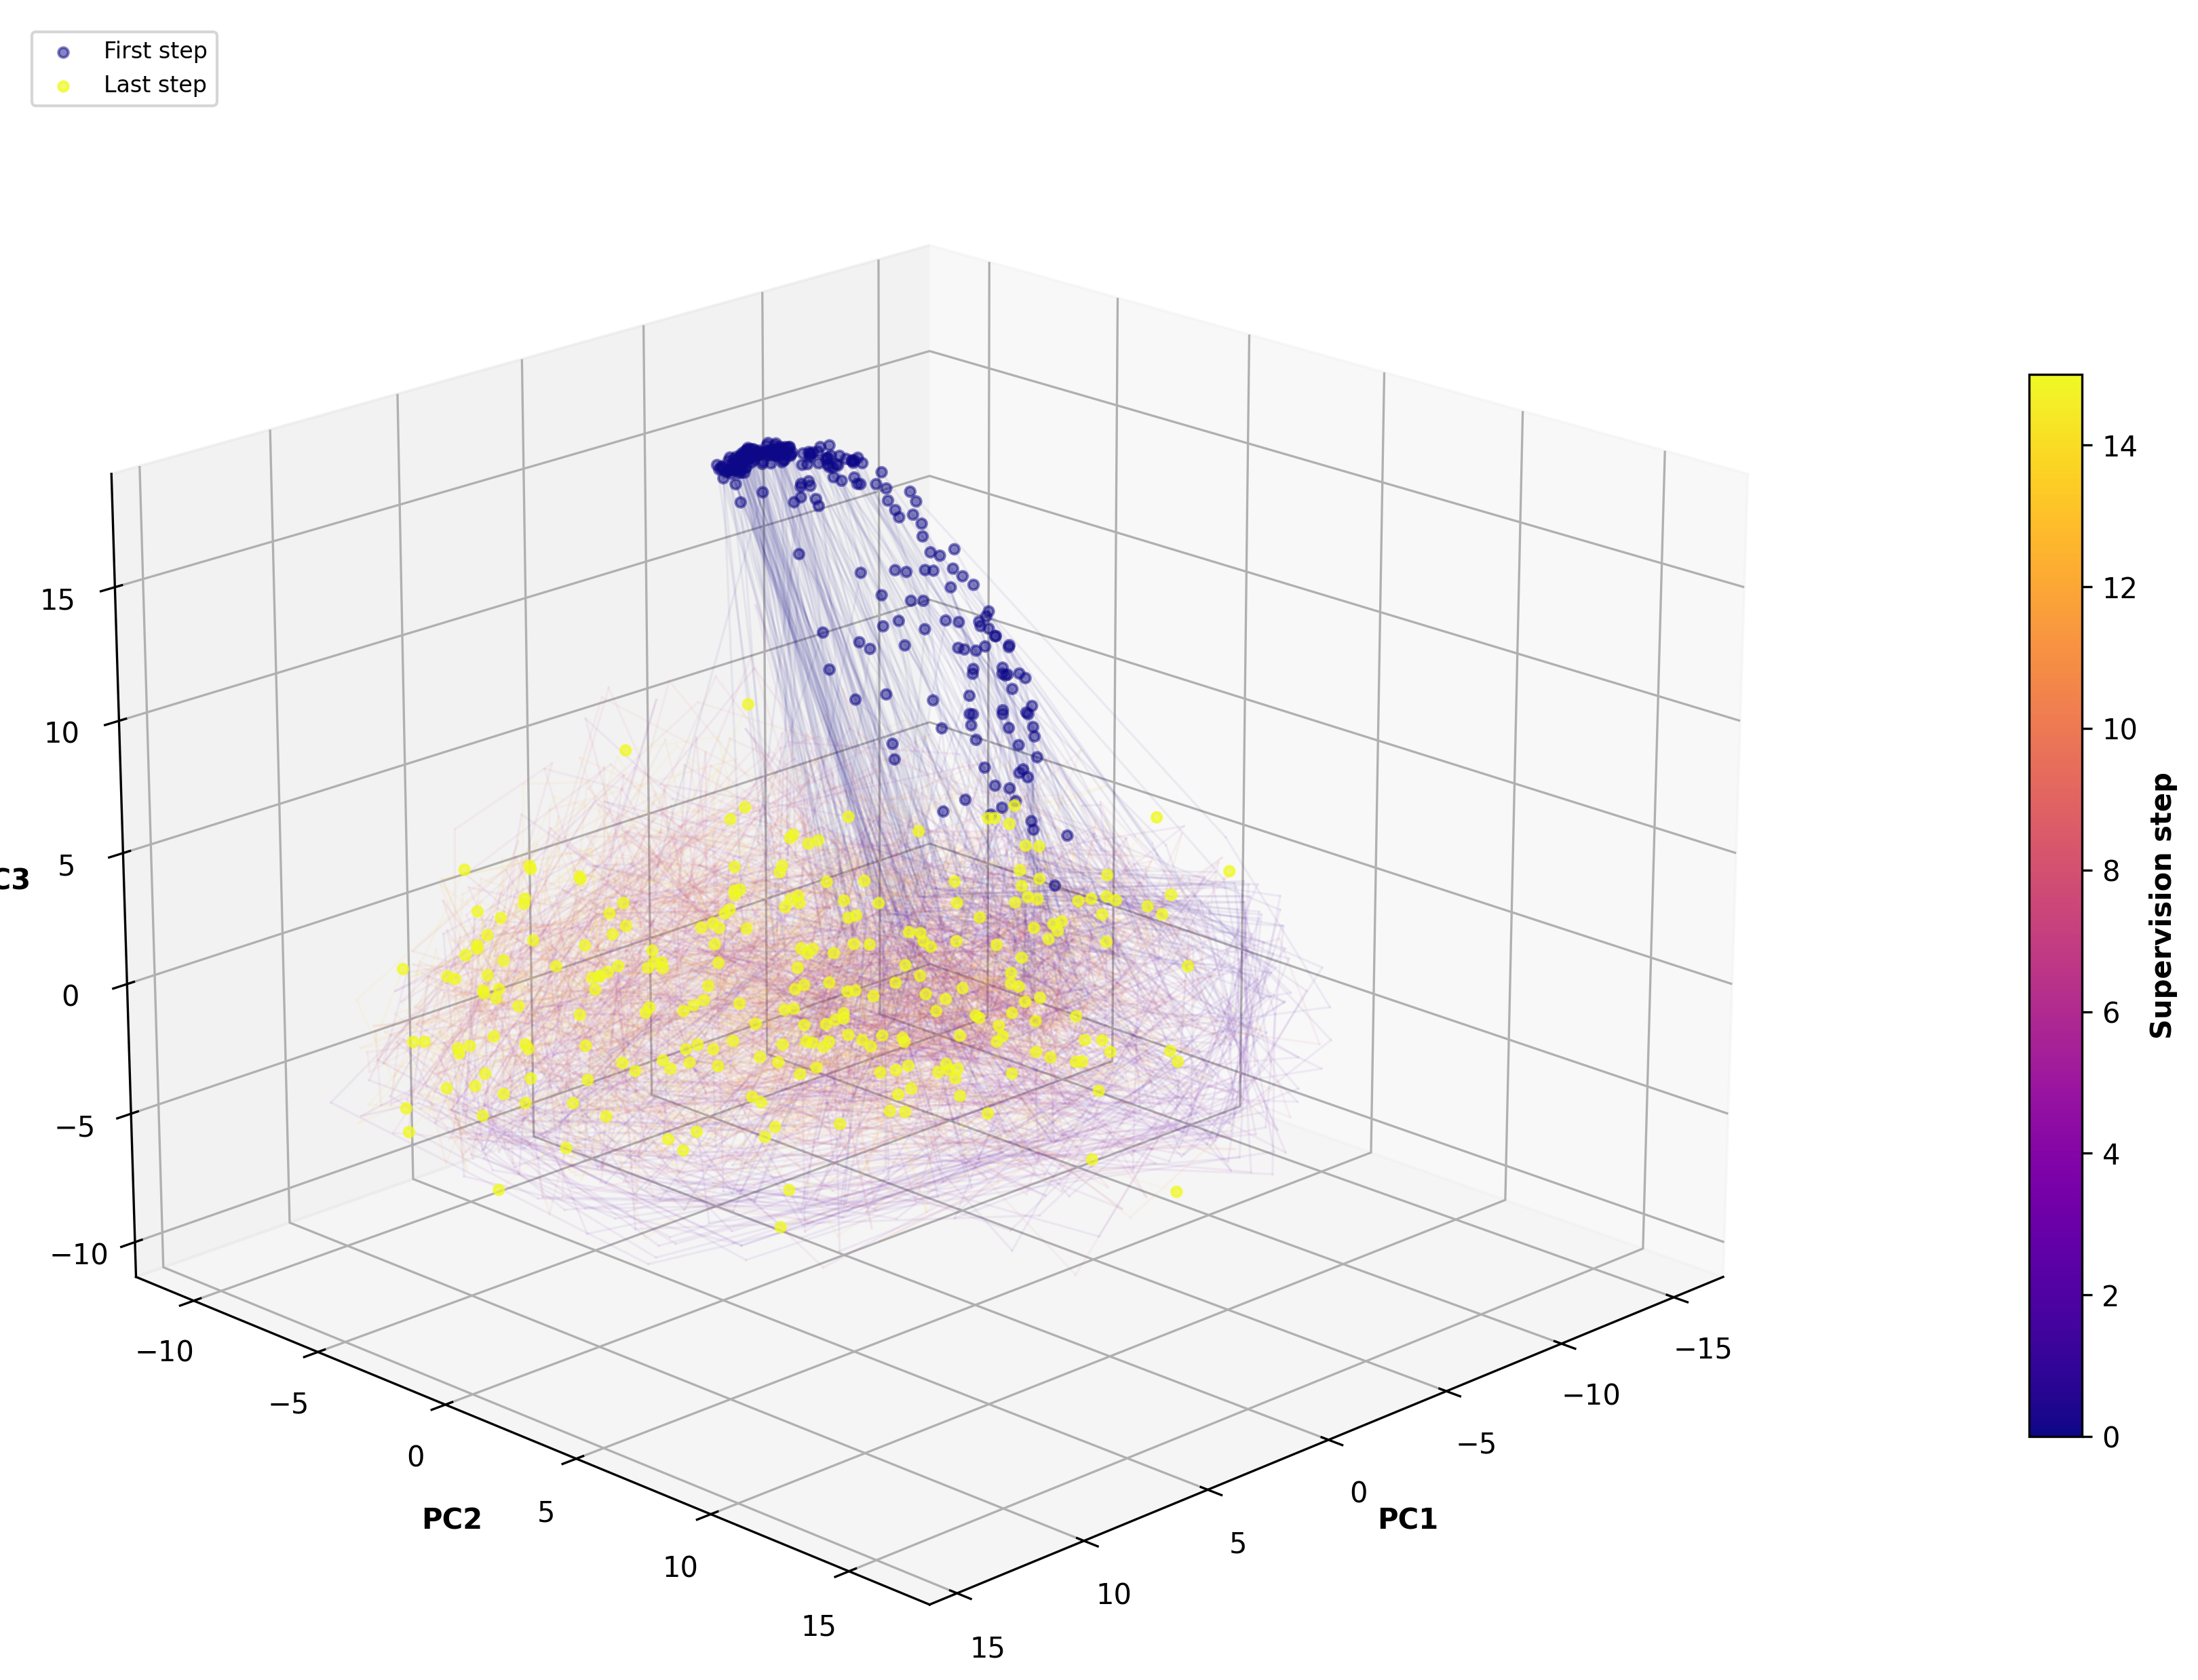
\includegraphics[width=0.73\textwidth]{./figures/agi_clusters.png}
    \captionof{figure}{ARC-AGI v1 clusters}
    \label{fig:agi-v1-clusters}

    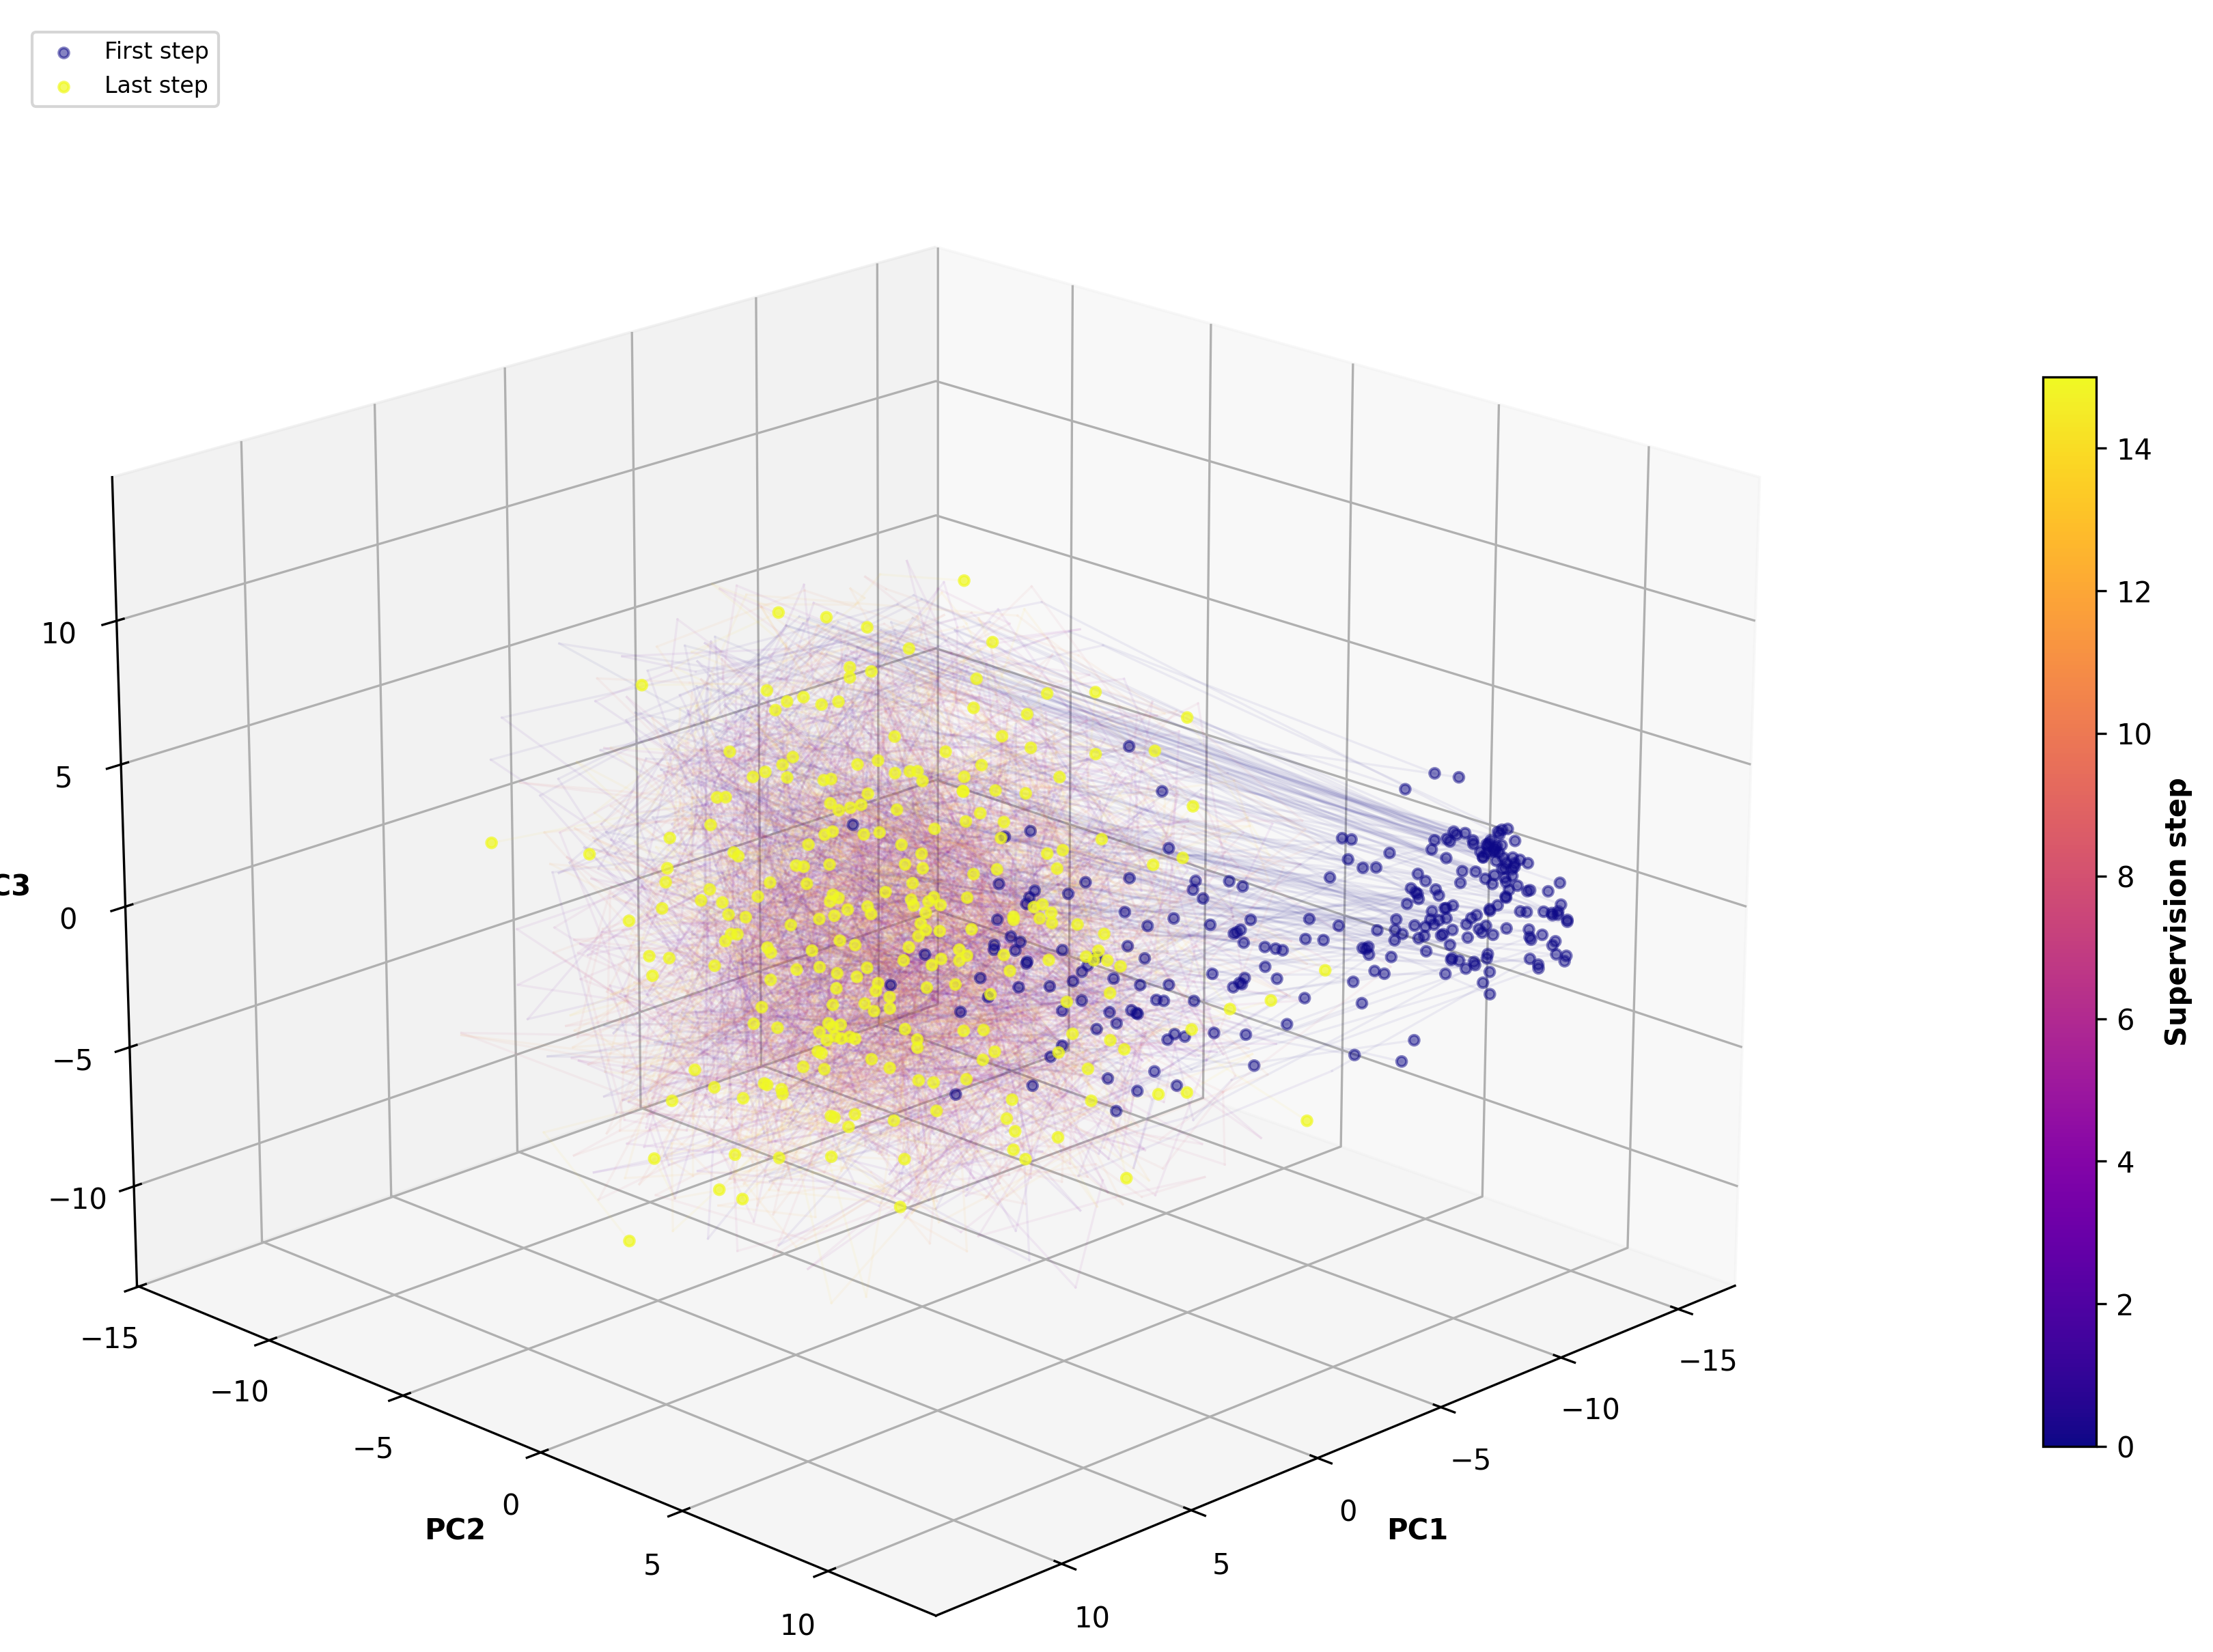
\includegraphics[width=0.73\textwidth]{./figures/agi2_clusters.png}
    \captionof{figure}{ARC-AGI v2 clusters}
    \label{fig:agi-v2-clusters}
\end{center}


\subsubsection*{Sample Trajectories}

The following plots show the trajectory of a randomly selected sample, projected into a compressed 3D space, with the goal of visualizing the path followed by the latent solution across supervision steps.
The trajectory of $y$ is averaged across tokens to obtain a global representation at each step, then subsampled every $4$ steps to retrieve the $y$ values corresponding to the $N_{sup}=16$ supervision steps.
Unlike the previous analysis, here the PCA is fitted only on the points of this individual trajectory, projecting it independently into a 3D space to visualize its specific path. Alongside the trajectory, we report the standard and normalized acceleration (Equations~\ref{eq:acceleration} and~\ref{eq:norm-acceleration}), computed from consecutive differences $\Delta^{(k)}$, with the supervision step encoded by color in both plots.

\begin{center}
    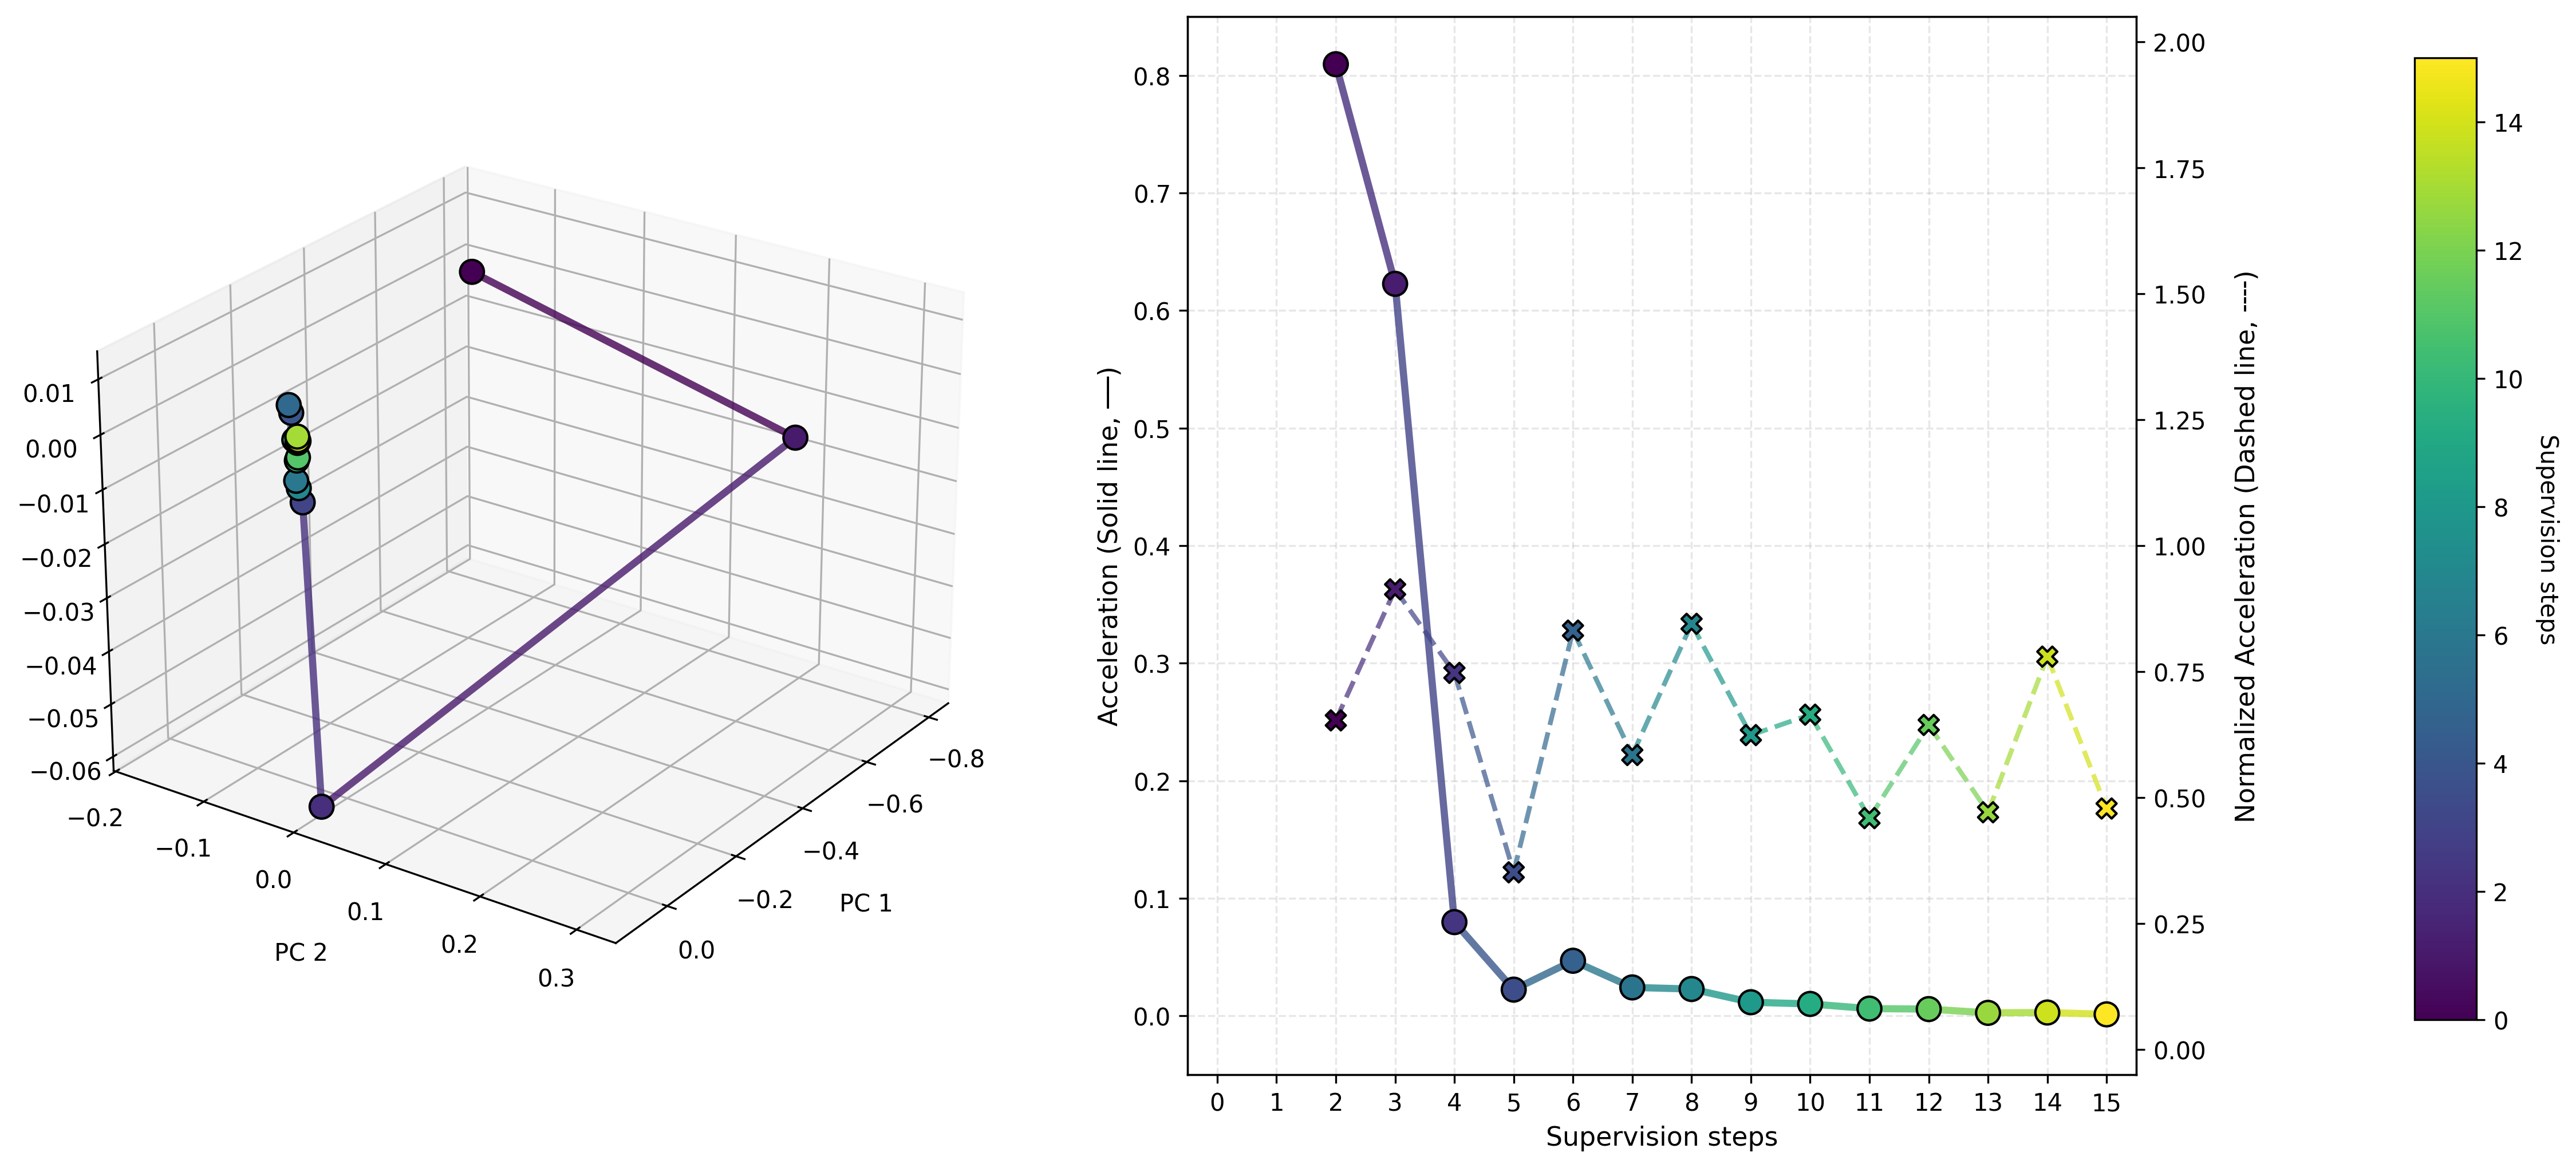
\includegraphics[width=\textwidth]{./figures/maze5x5_sample-traj.png}
    \captionof{figure}{Maze 5x5 sample trajectory}
    \label{fig:maze5x5-traj}

    \vspace{1cm}

    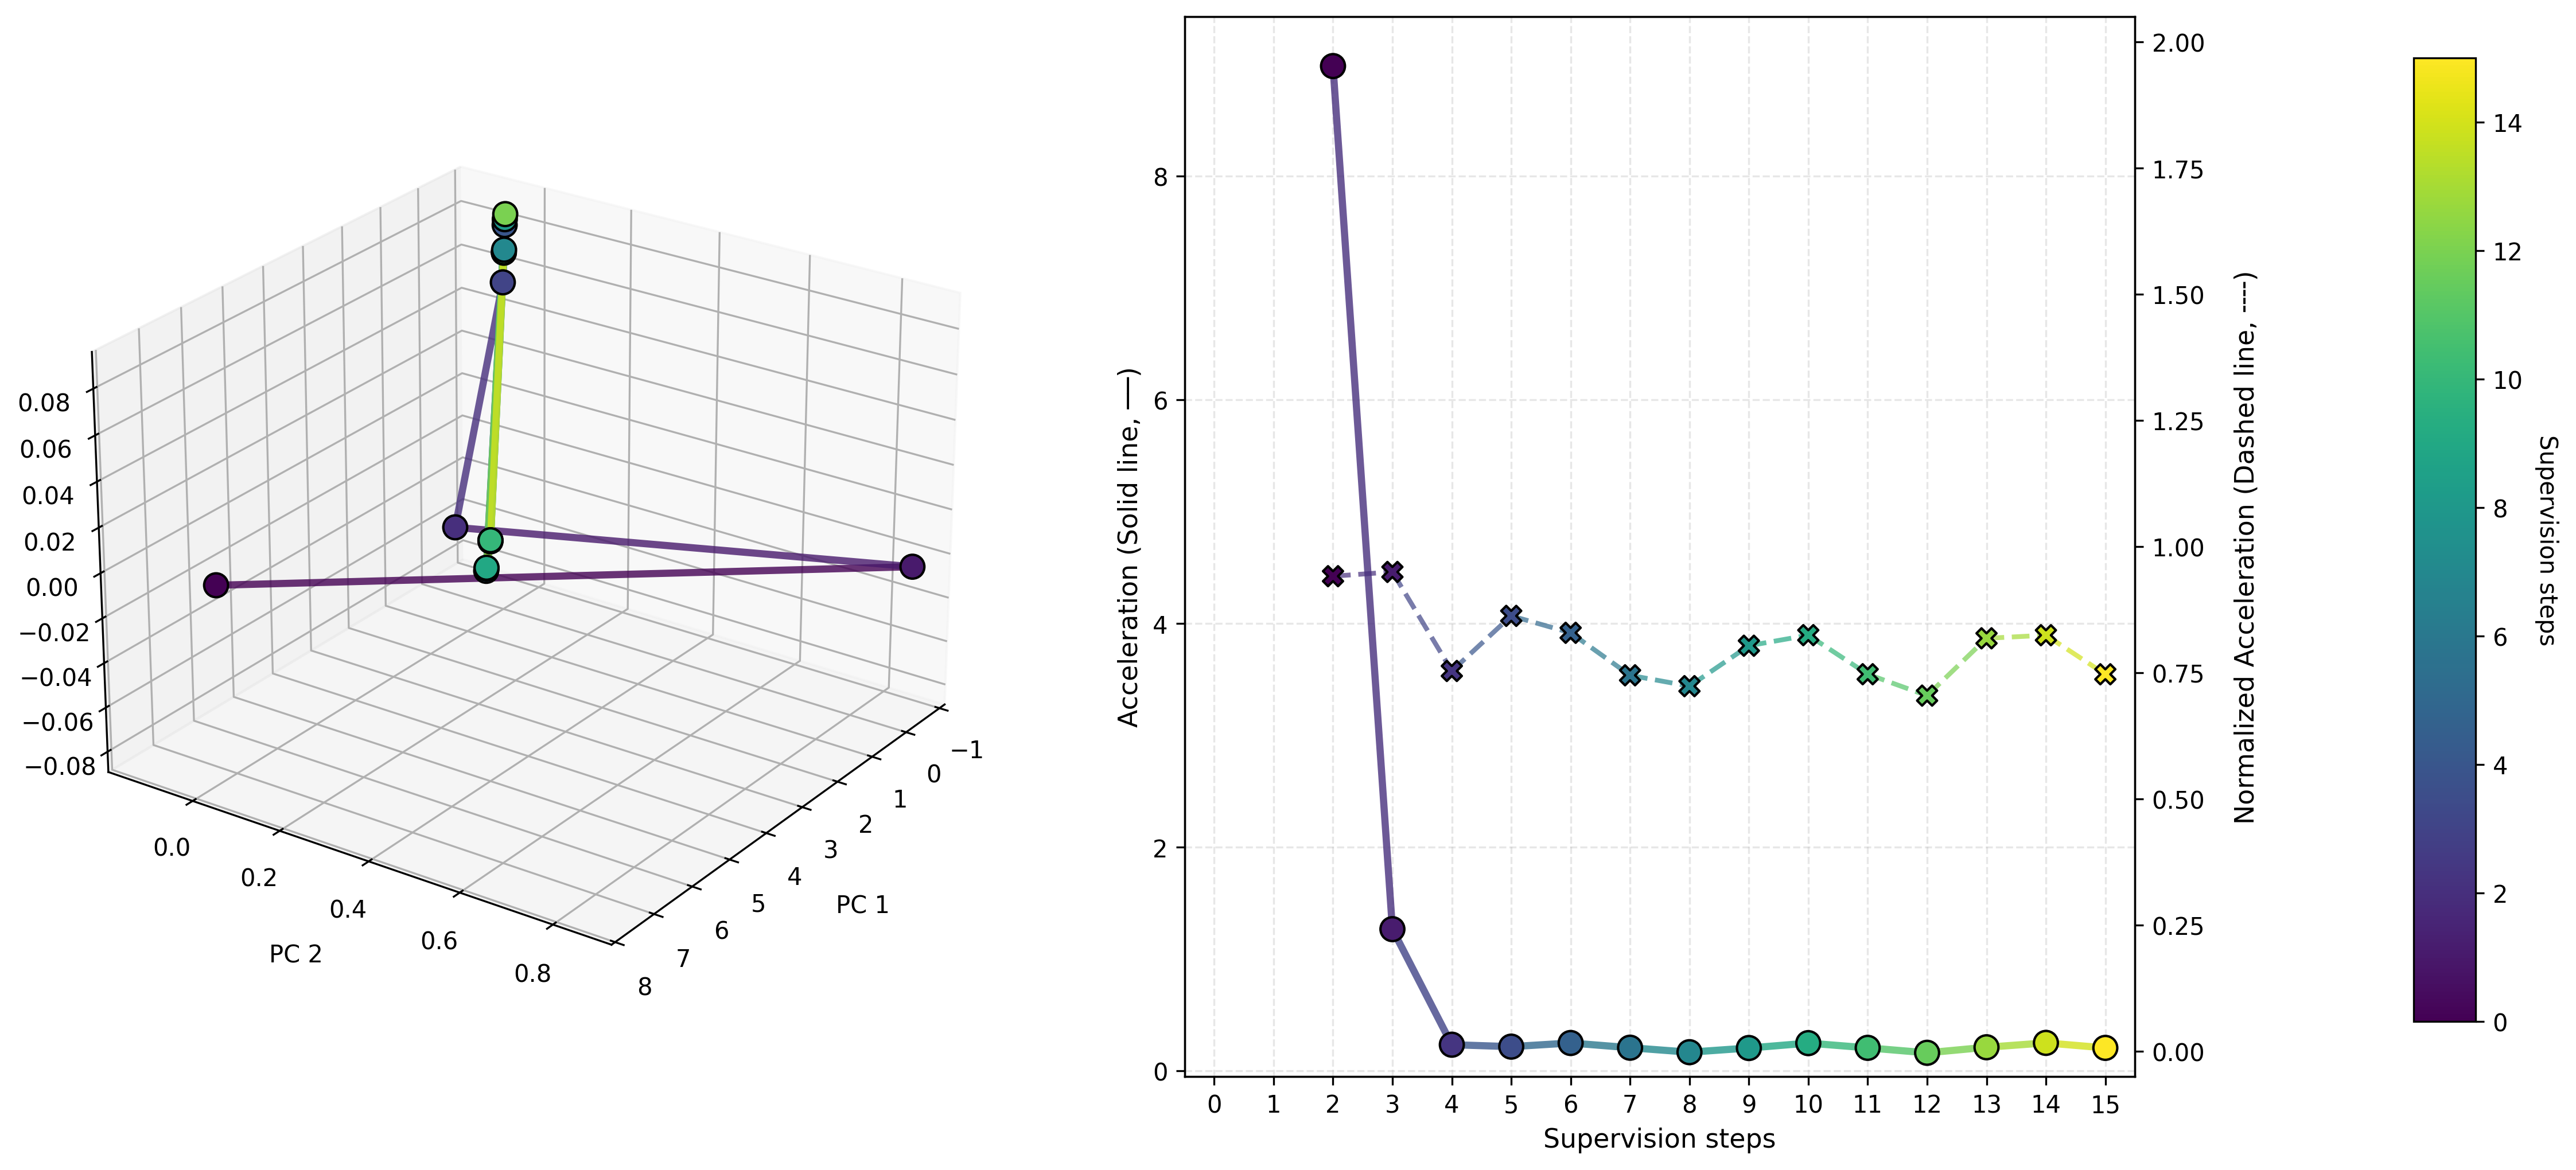
\includegraphics[width=\textwidth]{./figures/sudoku9x9-attn_sample-traj.png}
    \captionof{figure}{Sudoku 9x9 (attn) sample trajectory}
    \label{fig:sudoku9x9-traj}
\end{center}

\end{document}

